\documentclass[11pt]{article}

%LISTE DES PACKAGES
\usepackage[T1]{fontenc}
\usepackage[utf8]{inputenc}
\usepackage[english]{babel}
\usepackage{fancyhdr, graphicx, soul}
\usepackage[left=2cm,right=2cm,top=2cm,bottom=3cm]{geometry}
\usepackage{lastpage}% Pour la référence de dernière page
\usepackage{ulem}
\usepackage{array}
\usepackage{float}
\usepackage{xcolor}
\usepackage{pifont}
\usepackage{lipsum}%générateur de texte
\usepackage{amsmath}%math
\usepackage[hidelinks]{hyperref}%références url
\usepackage{biblatex} %Imports biblatex package
\usepackage{indentfirst}
\setlength{\parindent}{5ex}
\addbibresource{references.bib} %Import the bibliography file
\usepackage{caption}
\usepackage{subcaption}
\usepackage{tabularx}
\usepackage{booktabs}
\usepackage{tikz}
\usetikzlibrary{positioning}

%put code snippet
\usepackage{listings}
\definecolor{codegreen}{rgb}{0,0.6,0}
\definecolor{codegray}{rgb}{0.5,0.5,0.5}
\definecolor{codepurple}{rgb}{0.58,0,0.82}
\definecolor{backcolour}{rgb}{0.95,0.95,0.92}

\lstdefinestyle{mystyle}{
	backgroundcolor=\color{backcolour},   
	commentstyle=\color{codegreen},
	keywordstyle=\color{magenta},
	numberstyle=\tiny\color{codegray},
	stringstyle=\color{codepurple},
	basicstyle=\ttfamily\footnotesize,
	breakatwhitespace=false,         
	breaklines=true,                 
	captionpos=b,                    
	keepspaces=true,                 
	numbers=left,                    
	numbersep=5pt,                  
	showspaces=false,                
	showstringspaces=false,
	showtabs=false,                  
	tabsize=2
}

\lstset{style=mystyle}

%MISE EN FORME PAGE DE TITRE
\fancypagestyle{thetitlepage}{
	\fancyhead{} % clear all header fields
	\fancyhead[RO,LE]{
\includegraphics[scale=0.4]{img/logo.pdf}}
	\fancyhead[RE,LO]{Bern University of Applied Sciences} 
	\fancyfoot{} % clear all footer fields
	\renewcommand{\headrulewidth}{0pt}
	\renewcommand{\footrulewidth}{0pt}}

%EN-TETE ET PIED DE PAGE
\fancypagestyle{theotherpages}{
	\renewcommand{\headrulewidth}{0.5pt}
	\fancyhead[L]{University of Bern}
	\fancyhead[R]{}
	\renewcommand\footrulewidth{0.5pt}
	\fancyfoot[L]{Technology and Diabetes Management}
	\fancyfoot[C]{ Diabetes prediction}
	\fancyfoot[R]{\thepage\ / \pageref{LastPage}}}

%Modifie la hauteur des lignes des tableaux
\renewcommand{\arraystretch}{1.3}

% Set table of context depth to subsections
%\setcounter{secnumdepth}{2}
%\setcounter{tocdepth}{2}


\begin{document}
	% CONTENU  PAGE DE TITRE
	\begin{titlepage}
		\thispagestyle{thetitlepage}
		\begin{center}
			\vspace*{2cm}
			
			\Huge{- Project 1: Diabetes prediction -}
			
			\vspace{0.5cm}
			
			\begin{table}[H]
				\renewcommand{\arraystretch}{1.3}
				\centering	
				\begin{tabular}{|l|l|}
					\hline
					\Large{Author} & \Large{Daniel Monti \& Daniel Bürgler \& Camille Serquet} \\
					\hline
					\Large{Date} & \Large{\today} \\
					\hline
					\Large{Course} & \Large{D101722-HS2021-0: Technology and Diabetes Management } \\
					\hline
					\Large{Professor} & \Large{Stavroula Mougiakakou, PhD} \\
					\hline
					\Large{Assistant} & \Large{Matthias Fontanellaz, MSc, PhD Fellow} \\
					\hline
				\end{tabular}
			\end{table}
		\end{center}
		\vspace{0.7cm}
		\tableofcontents		
	\end{titlepage}
	
	\pagestyle{theotherpages}
	
	%%%%%%%%%%%%%%%%%%%%%%%%%%%%%%%%%%%%%%%%%%%%%
	\section{Introduction}
	Diabetes is a chronic metabolic disease associated with hyperglycemia. The chronic hyperglycemia results from defects in insulin secretion, insulin action, or both. Over time, diabetes leads to serious damage to the heart, eyes, kidney, nerves, and heart vessels. The prediction at an early stage of such a disease leads to improved treatment and mitigate the risk of long-term complications. Prediction Analysis uses statistics to create models that examine current and past data and predict potential future outcomes. When applied in health care, Prediction Analysis can help determine the patient’s risk of developing certain disease such as diabetes. It is therefore used as a tool to support medical decision-making and eliminate human efforts by supporting automation with minimum flaws \hl{[reference]}. In current medical diagnosis method, three types of errors are still to be \hl{deplored}: false-negative, false-positive, and unclassified type.	
	\bigbreak
	Classification algorithms need to be evaluated with evaluation metrics. The resulting accuracy gives a good appreciation of the algorithm and helps to detect which one suits best for a medical application. In this paper, the Pima Indian Diabetes Database \cite{Pima} is prepared and applied to classification algorithms such as Logistic Regression, Naïve Bayes, Stochastic Gradient Descent, K-Nearest Neighbors, Decision Tree, and Support Vector Machine. All algorithms will be reviewed. Finally, a comparison between all algorithms’ evaluation metrics will be evaluated.
	
	\section{Related work}
	There is currently considerably research being done on diabetes prediction with machine learning algorithms. This paper compares the six most common and traditional machine learning methods. However, more algorithms and methods are being developed to help predict diabetes. For instance, \citeauthor{POLAT2007702} \cite{POLAT2007702} use a principal component analysis (PCA) and neuro fuzzy inference. Other studies use ensemble methods to improve the accuracy of their results. \citeauthor{OZCIFT2011443} \cite{OZCIFT2011443} proposed an ensemble approach called rotation forest. It combines 30 machine learning methods. A quantum particle swarm optimization (QPSO) algorithm and weighted least squares support vector machine (WLS-SVM) was introduced by \citeauthor{Chen} to predict diabetes type 2. \citeauthor{Duygu} \cite{Duygu} proposed a new system called LDA-MWSVM. This system used Linear Discriminant Analysis (LDA) to reduce the dimensions and extract the features. To deal with the high dimensional datasets, \citeauthor{Razavian} \cite{Razavian} built prediction models based on logistic regression for different onsets of type 2 diabetes prediction. \citeauthor{Georga} \cite{Georga} focused on glucose and used support vector regression (SVR) to predict diabetes, which is a multivariate regression problem.

	\section{Methods}
	\subsection{Programming Language and used packages}
		This project is coded with Python version 3.9.9. the used packages can be seen in table \ref{tab:Python}.
	\begin{table}[H]
		\renewcommand{\arraystretch}{1.3}
		
		\centering
		\begin{tabularx}{\linewidth}{llX}
			Python Package & Version & Description \\
			\toprule
			NumPy \cite{numpy} & 1.21.4 & NumPy is the fundamental package for array computing with Python.\\
			pandas \cite{pandas} & 1.3.4 & pandas is a fast, powerful, flexible and easy to use open source data analysis and manipulation tool\\
			matplotlib \cite{matplotlib} & 3.5.0 & Matplotlib is a comprehensive library for creating static, animated, and interactive visualizations in Python\\
			seaborn \cite{seaborn} &  0.11.2 & Seaborn is a library for making statistical graphics in Python \\
			scikit-learn \cite{scikit} & 1.0.1  & scikit-learn is a Python module for machine learning built on top of SciPy \\

		\end{tabularx}
		\caption{Used Python libraries}
		\label{tab:Python}
	\end{table}
	The source code for this project is hosted on GitHub and is openly available on the following webpage: \url{https://github.com/d-monti/diabetesPrediction}.

	
	% Decision Tree
	\subsection{Decision Tree}
	Decision Tree is a tree-like model that contains conditional control statements. Each internal node represents a “test” on an attribute, each branch represents the outcome of the test, and each leaf represents the outcome (a final decision). The splitting criterion at a decision node is generated by Attribute Selection Measure (ASM).
	\medbreak
	Decision Tree algorithm has multiple advantages as it does not require the normalization of data nor the scaling of tha data, and the missing values do not affect the building process of the decision tree. Some drawbacks are the long time needed for training the model and the instability caused by a small change in the data.
	\medbreak
	The chosen model is the DecisionTreeClassifier. All default parameters are kept as so.
	The generation of the evaluation metrics gives an accuracy of [put result].
	
	\hl{Best Parameters are:  criterion: gini, splitter: best, max\_feature: log2, class weight balanced}

	
	% K-Nearest Neighbours
	\subsection{K-Nearest Neighbours}
	K-Nearest Neighbors (KNN) based classification is a type of instance-based learning or non-generalizing learning. The algorithm does not attempt to construct an internal model but instead stores training data instances. It then classifies the new point by a majority vote of the k-nearest neighbours. The optimal choice for the k-factor depends on the data itself. In general, a larger k suppresses noise but makes the classification boundaries less distinct. Since KNN relies on the distance to classify, the data was normalized beforehand. Normalization was chosen over standardization since the algorithm parameters p were left at its default = 2 and the metric, which is 'minkowski'. This is equivalent to the standard Euclidean metric. The ideal parameters were found to achieve the highest accuracy by using the GridSearch() function and 5-fold cross-validation. A Grid from 1-30 for the k-value was created, and different leaf\_sizes, algorithms and weights were checked. The highest precision was found with a k-neighbor size of 21, algorithm = 'auto', leaf\_size = 10, weights = 'distance'. The leaf\_size is passed to the algorithms BallTree or KDTree. This can affect the speed of the construction and the memory, which is required to store the tree. The weights were selected as 'distance', which means that closer neighbours of a query point will have a greater influence than further away neighbours.
		
	% Logistic Regression
	\subsection{Logistic Regression}
	Logistic regression (LR) is one of the most used machine learning algorithms for binary classification problems. LR is a linear method, but the predictions are transformed using the logistic(sigmoid) function. An optional L1, L2 or Elastic-Net regularization can be applied. It is also commonly referred to as a penalized logistic regression. Using a penalty is favourable as they solve optimization problems to achieve a good result and improve numerical stability. The Elastic-Net is a combination of both L1 and L2.  No regularization amounts to setting C to a very high value. C is the inverse of regularization strength. Hence smaller values specify stronger regularization.
	To achieve the highest accuracy and find the optimal parameters/hyperparameters for the LR algorithm, a randomized search approach with 5-fold cross-validation was used. The randomized search approach was used. Furthermore, a comparison between standardized scaled and unscaled data was made. The scaled data consistently achieved a higher accuracy of roughly 1\% compared to the unscaled data. The highest accuracy was found using the L1 penalty with the 'saga' solver. The found C value with random search lies at 0.33. This indicates a strong regularization. Since all classes should have equal weight, the weight\_class parameter was kept at the default value 'balanced'. It is essential to state that the retrieved parameters can change with each code compilation since a random search was used.
	
	% Naïve Bayes
	\subsection{Naïve Bayes}
	Naive Bayes (NB) is a probabilistic classification technique based on Bayes’ theorem with the assumption of independence between all features in a class. Bayes’ theorem gives the probability that an event happens with the knowledge of another event with the condition that they are not interdependent. In a Gaussian Naive Bayes classifier, each values are continuous and assumed to be normally distributed.
	\medbreak
	NB is a good classifier when it comes to multi-class prediction dataset and when the independence between all classes remains true. One big advantage of NB is that it requires a small amount of training data to estimate the test data which leads to a short training period. A drawback of this implementation is the assumption of independent predictors which, in real life, is almost impossible to achieve. 
	\medbreak
	The chosen model is the GaussianNB(). Both parameters \textit{priors} and \textit{var\_smoothing} are kept as default. The generation of the evaluation metrics gives an accuracy of [put result].

	
	% Support Vector Machine
	\subsection{Support Vector Machines}
	Support vector machines (SVMs) are supervised learning methods used for classification, regression, and outliners detection.
	\medbreak
	An advantage of SVMs is that it is effective in high dimensional spaces, even in cases where the number of dimensions is greater than the number of samples. SVMs are also memory efficient because they use a subset of training points in the decision function (called support vectors). Another advantage is that SVMs is versatile in which different Kernel functions can be specified for the decision function.
	One disadvantage of SVMs is that if the number of features is much greater than the number of samples, the choice of Kernel functions and the regularization term become crucial to avoid overfitting. Another drawback is that SVMs do not directly provide probability estimates; these are calculated using time expensive k-fold cross-validation.
	\medbreak
%	\hl{remove if to many pages}
%	In the SVMs model we can chose between the following four kernel functions, the figure \ref{fig:svms} illustrates the differences between the kernels.
%	
%	\begin{minipage}[b]{0.5\linewidth}
%		\begin{table}[H]
%			\begin{tabularx}{\textwidth}{lX}
%				Linear & $\left\langle x, x^{\prime}\right\rangle$\\
%				Rbf &  $\exp \left(-\gamma\left\|x-x^{\prime}\right\|^{2}\right)$, where $\gamma$ is specified by parameter gamma \\
%				Polynomial & $ \left(\gamma\left\langle x, x^{\prime}\right\rangle+r\right)^{d}$, where $d$ is specified by parameter degree, $r$ by coefo  \\
%				Sigmoid & $\tanh \left(\gamma\left\langle x, x^{\prime}\right\rangle+r\right)$, where $r$ is specified by coefo \\
%			\end{tabularx}
%			\caption{Support Vector Machines Kernels}
%			\label{tab:svmsKernels}
%		\end{table}
%	\end{minipage}
%	\begin{minipage}[b]{0.5\linewidth}
%			\begin{figure}[H]
%			\centering
%			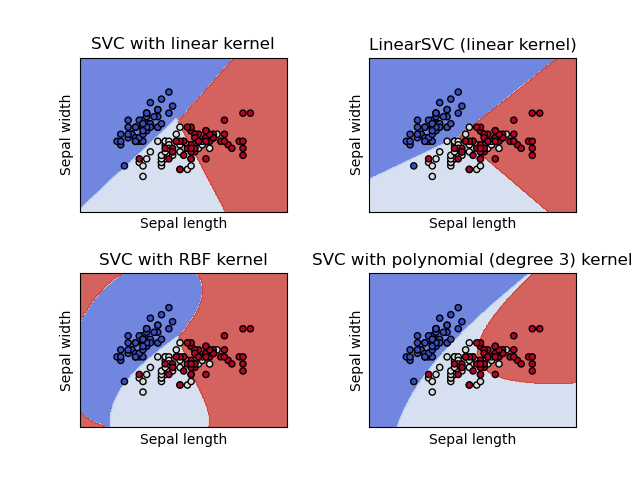
\includegraphics[width=0.8\textwidth]{img/svms}
%			\caption{Support Vector Machines Kernels \cite{scikit}}
%			\label{fig:svms}
%		\end{figure}
%	\end{minipage}
	For this model the dataset will be tested scaled and non scaled, this means training an SVMs over the scaled and non-scaled data leads to the generation of different models. To tune the SVMs model the following parameters where tested with a grid search and cross validation with 5 time folding. The underlined parameters are the best-performing ones, and we used them in this project. The scaled test dataset was used, because it scored a higher accuracy. The best parameters can vary for every run of the source code.
	\begin{table}[H]
		\renewcommand{\arraystretch}{1.3}
		\centering
		\begin{tabular}{llllll}
			Kernel & C  & gamma & class\_weight & coef0 & degree \\
			\toprule
			Linear & 0.9, 1, 2, 10  & & balanced & & \\
			\underline{Rbf} &  0.9, \underline{1}, 2, 10  & \underline{scale}, auto & \underline{balanced} & & \\
			Polynomial & 0.9, 1, 2, 10 & scale & balanced & 0.0 & 2, 3, 4, 5, 6, 7 ,8 \\
			Sigmoid & 0.9, 1, 2, 10  & scale, auto & balanced & & \\
		\end{tabular}
		\caption{Support Vector Machine grid search used test parameters}
		\label{tab:SVMSParameters}
	\end{table}

	% Stochastic Gradient Descent
	\subsection{Stochastic Gradient Descent}
	Stochastic Gradient Descent (SGD) is a simple yet very efficient approach to fit linear classifiers and regressors under convex loss functions such as (linear) Support Vector Machines and Logistic Regression. Even though SGD has been around in the machine learning community for a long time, it has received a considerable amount of attention just recently in the context of large-scale learning.
	\medbreak
	The advantages of Stochastic Gradient Descent are its efficiency and the ease of the implementation with a lots of opportunities for code tuning. One drawback of SGD is that its requires a number of hyperparameters such as the regularization parameter and the number of iterations. SGD is also sensitive to feature scaling, and therefore this model was tested with the scaled and non scaled dataset. This model has a lot of parameter to test, following a list of all tested parameters. The underlined parameters are the best-performing ones, and we used them in this project. The scaled test dataset was used, because it scored a higher accuracy. The best parameters can vary for every run of the source code.
	
	\begin{table}[H]
		\renewcommand{\arraystretch}{1.3}
		\centering
		\begin{tabularx}{\textwidth}{lX}
			Parameters & Values \\
			\toprule
			loss &  hinge, log, modified\_huber, squared\_hinge, perceptron, squared\_error, huber, \underline{epsilon\_insensitive}, squared\_epsilon\_insensitive\\
			penalty & l1, \underline{l2}, elasticnet   \\
			class\_weight & \underline{balanced}\\
			l1\_ratio & $0-1$ in 10 steps (best: \underline{0.0})\\
			alpha & $0.0001 - 0.1$ (best: \underline{0.01})\\
		\end{tabularx}
		\caption{Stochastic Gradient Descent grid search used test parameters}
		\label{tab:SGDParameters}
	\end{table}


%	\begin{figure}[H]
%		\centering
%		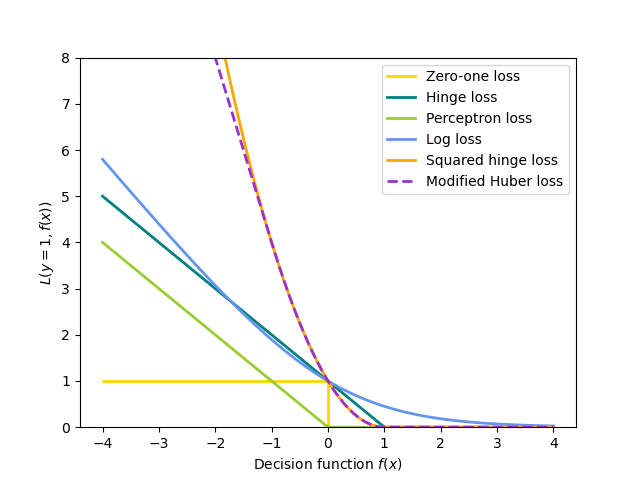
\includegraphics[width=0.8\textwidth]{img/sgd}
%		\caption{Support Vector Machines Kernels \cite{scikit}}
%		\label{fig:sgd}
%	\end{figure}
	
	\subsection{Cross Validation}
	The dataset needs to be split into a test dataset and a training dataset to train and test the machine learning models. In our case, the test dataset is 25\% of the entire dataset. We use the training dataset to fit the machine learning model and the test dataset to evaluate the machine learning model. We applied the cross-validation technique to resample the data accordingly. This means that different portions of the data are used to train and then evaluate the models with each iteration. We used fivefold cross-validation for our algorithms. The principle of data resampling can be seen in Figure \ref{fig:crossValidation}. We chose five as more iterations only slow down the overall code speed and does not significantly impact the results.
	\begin{figure}[H]
		\centering
		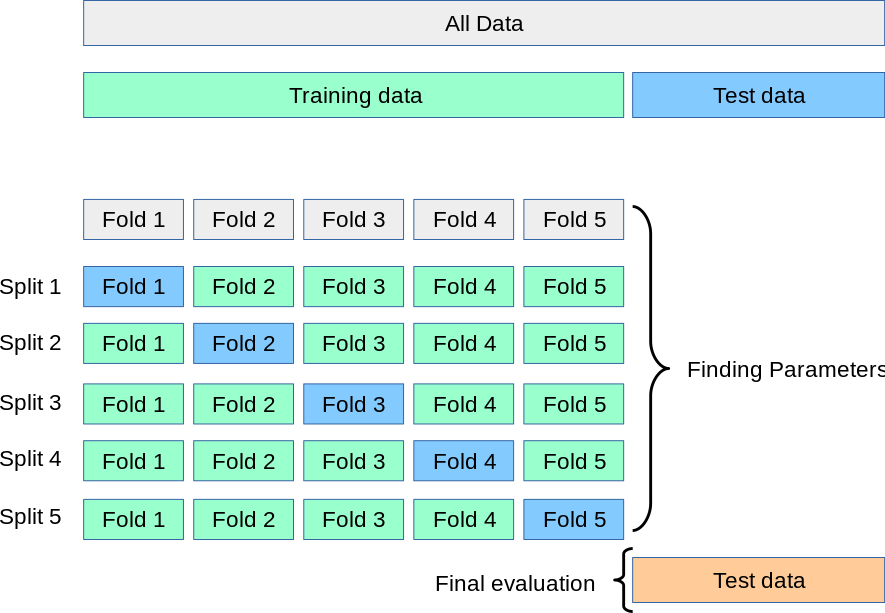
\includegraphics[width=0.5\textwidth]{img/grid_search_cross_validation.png}
		\caption{Fivefold Cross Validation \cite{scikit}}
		\label{fig:crossValidation}
	\end{figure}
	\subsection{Tuning Algorithms}
	The final accuracy score of the algorithms can be fined tuned by changing and adapting its parameters. Some parameters can be learned automatically, but hyper-parameters must be set manually. Setting the hyper-parameters is usually not clear and has to be searched with different methods. The algorithms SGD, SVMs, Decision Tree and KNN use the Grid Search, and the Random Search method is used for Logistic Regression. In Figure \ref{fig:tuningAlgos} the hyper-parameters and parameters are represented as dots, and the green curve above displays its respective model accuracy. The grid search is labelled as (a) and the Random Search as (b). The Random Search defines a search space as a bounded domain of hyperparameter values and randomly samples points in that domain. It has greater variability, and therefore changes in the hyperparameter can have a greater influence on the model tuning. On the other hand, the grid search defines a search space as a grid of hyperparameter values and evaluates every position in the grid.
	\begin{figure}[H]
		\centering
		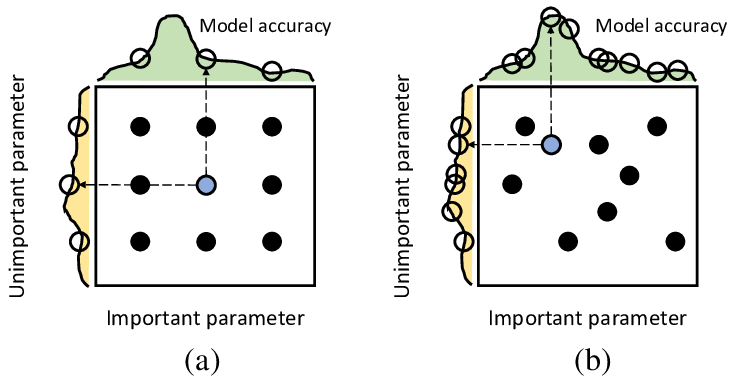
\includegraphics[width=0.5\textwidth]{img/gridsearchAndRandomsearch}
		\caption{Comparison between (a) Grid Search and (b) Random Search. Changing hyper-parameters has an influence on the model accuracy \cite{Pilario}}
		\label{fig:tuningAlgos}
	\end{figure}
	\subsection{Model Comparisons}
	To compare the models against each other, the best parameters are automatically chosen, and with them, another cross-validation with 5 times folding is done.
	The accuracy of all models is then used to create a boxplot, which allows us to compare the model against each other quickly. The accuracy only demonstrates to us a small part of the performance of a model. Therefore also the Specificity, Sensitivity and the F1 value are evaluated. Following the equations to get these values.
	$$ 
	\text{Specificity} = \frac{\text{True Negative}}{\text{True Negative} + \text{False Positve}} $$
	$$
	\text{Sensitivity} = \frac{\text{True Positive}}{\text{True Positive} + \text{False Negative}}
	$$	
	$$
	F_{1}=\frac{\text{True Positive}}{\text{True Positive} + \frac{1}{2}(\text{False Positve} + \text{False Negative})}
	$$
	\section{Data and Experiment setup}
		\subsection{Dataset}
	The Pima Indians Diabetes Database \cite{Pima} is used to build a model that accurately predict whether or not the patients in the dataset have diabetes or not. The datasets contains several medical predictor variables and one target variable; the output. All patients registered in this dataset are females, take part of the Pima Indian heritage, and are at least 21 years. The dataset contains 768 patients.
	\subsubsection*{Predictor variables and target variable of the dataset}
	\begin{itemize}
		\item \textbf{Pregnancies} : number of times pregnant
		\item \textbf{Glucose} : plasma glucose concentration a 2 hours in an oral glucose tolerance test
		\item \textbf{BloodPressure} : diastolic blood pressure (mmHg)
		\item \textbf{SkinThickness} : triceps skin fold thickness (mm)
		\item \textbf{Insulin} : 2-Hour serum insulin (muU/ml)
		\item \textbf{BMI} : Body mass index (weight in kg/(height in m)$^2$)
		\item \textbf{DiabetesPedigree} : diabetes pedigree function (A function that scores the likelihood of diabetes based on family history)
		\item \textbf{Age} : age (years)
		\item \textbf{Outcome} : class variables(0 or 1)
	\end{itemize}
	Multiple statistical tools allows a clear overview of the dataset. As some algorthm require the independancy of all variabels, the coorelation between them are calculated and shown in figure \ref{fig:datasetCorrelation}. The figure \ref{fig:datasetHistogram} show the histogram of the dataset. 
	
	\begin{figure}[H]
		\begin{minipage}[b]{0.5\textwidth}
			\centering
			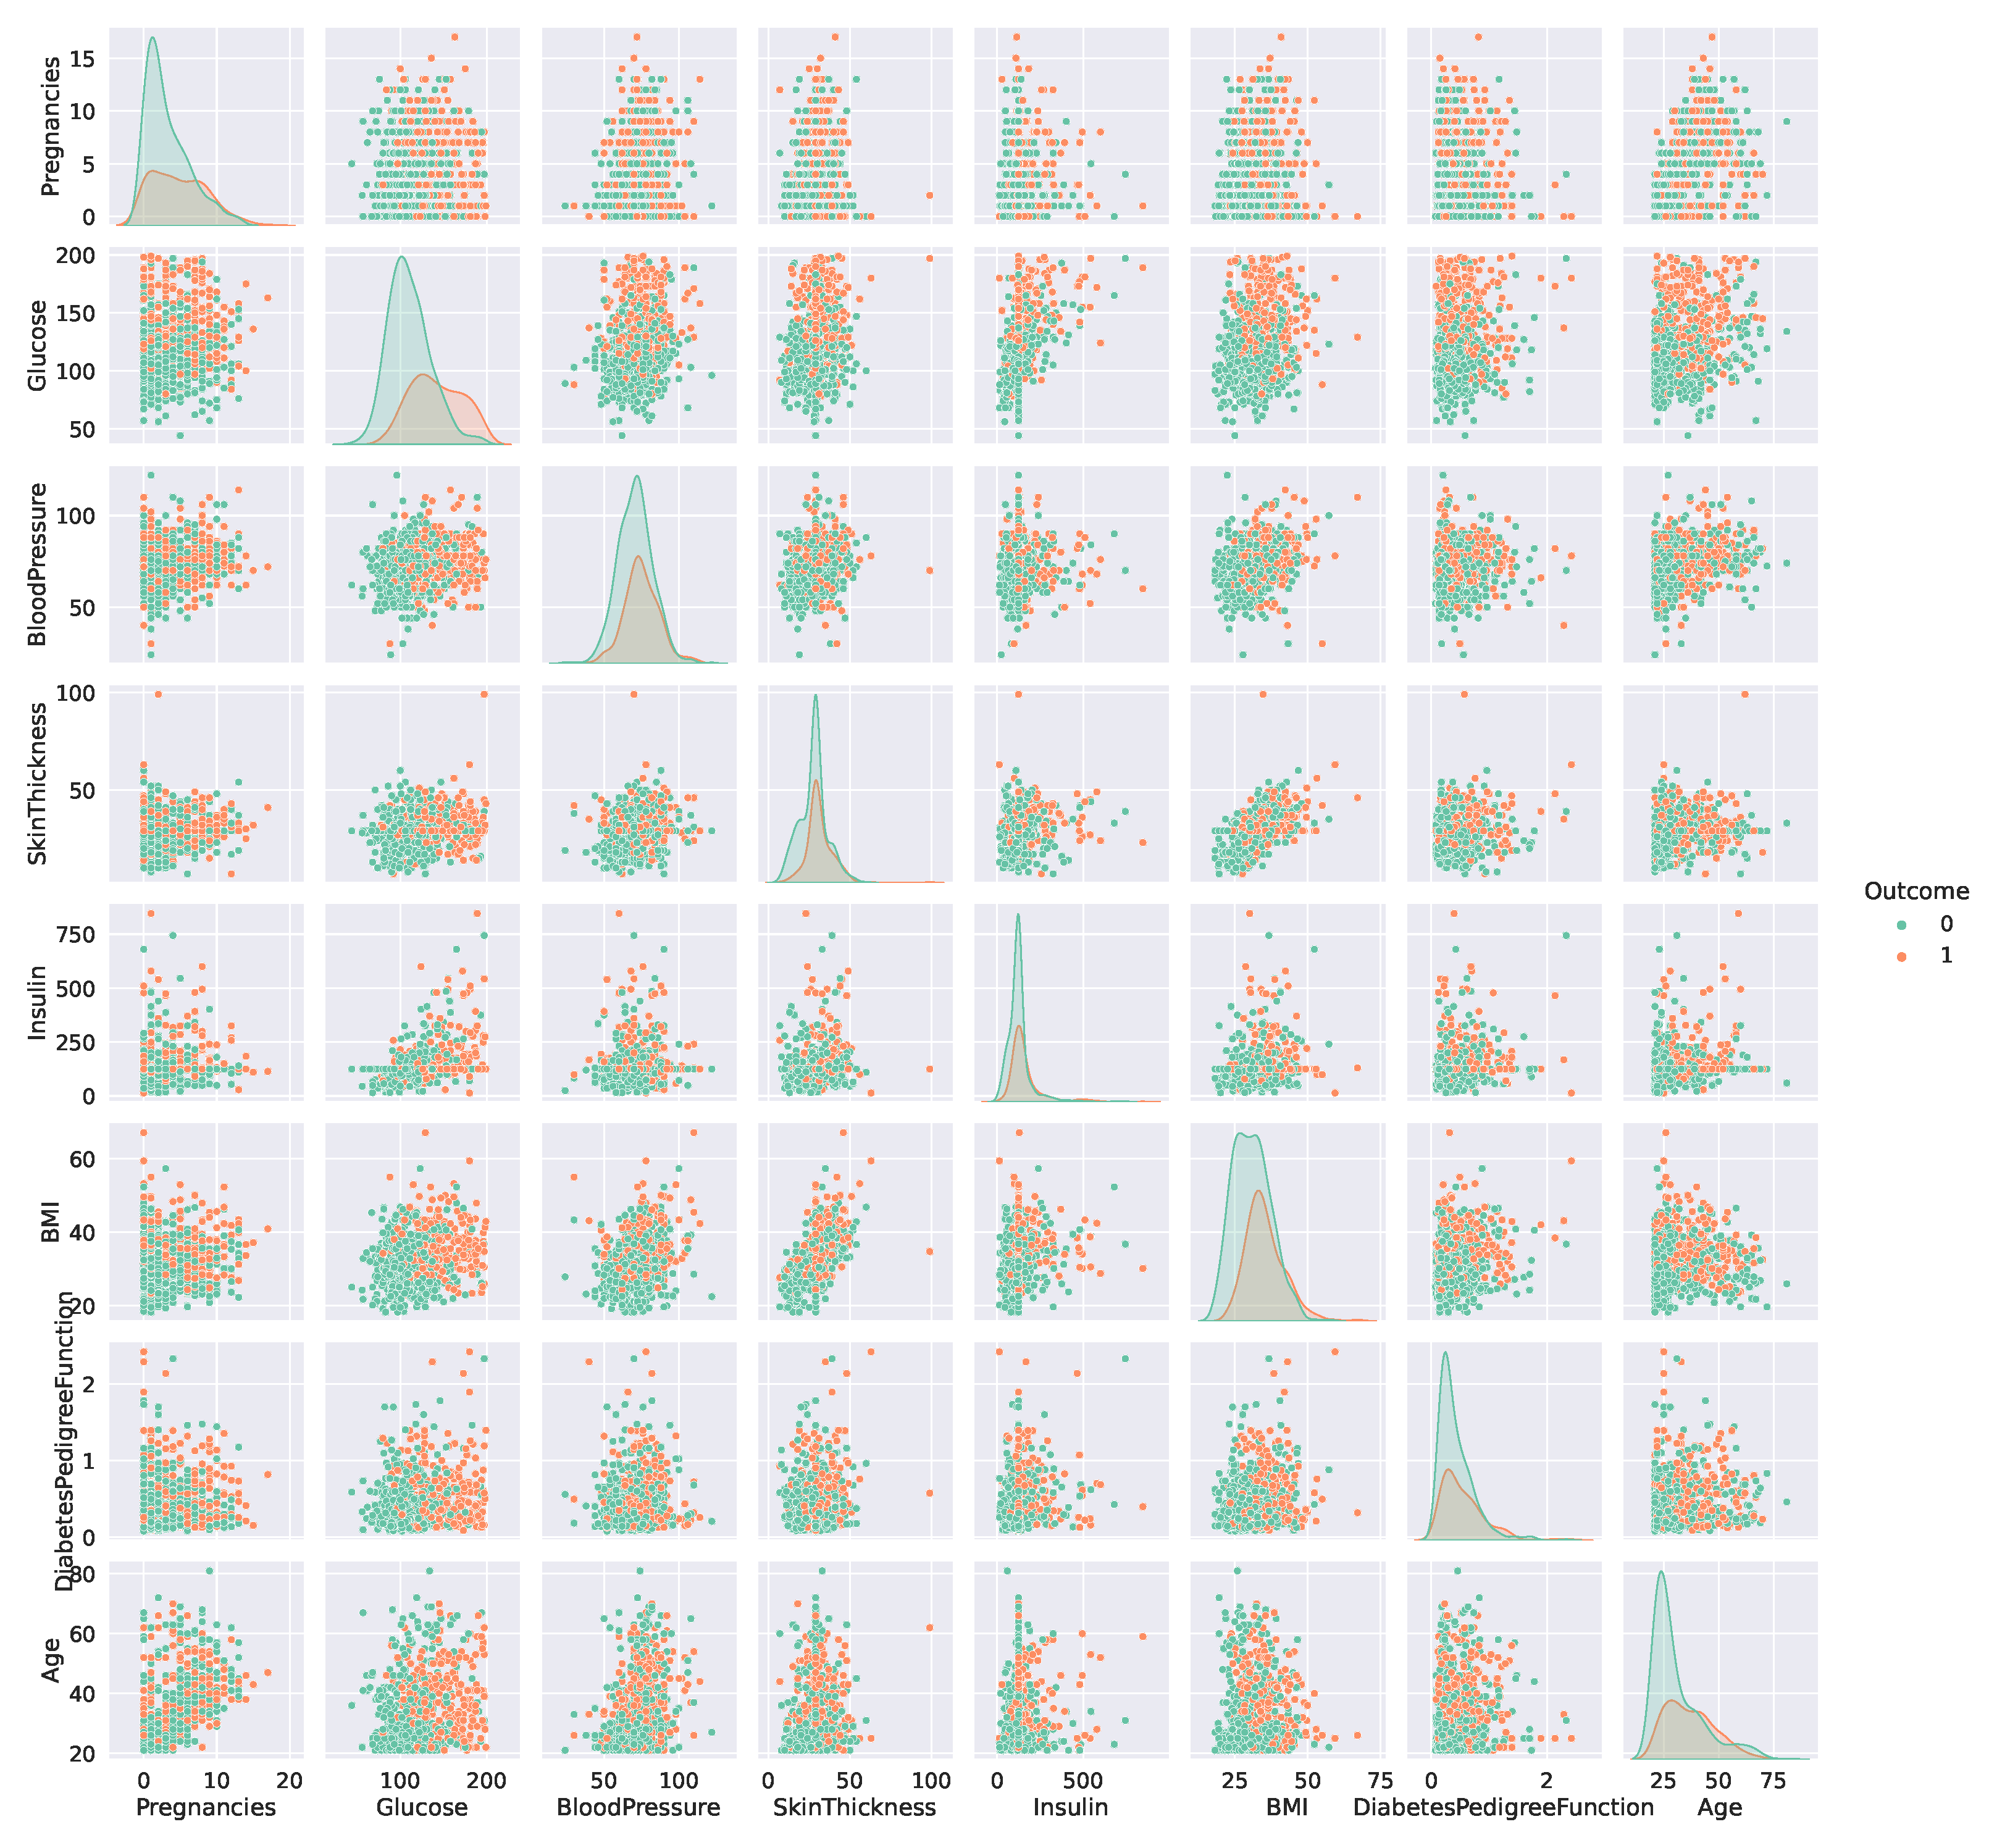
\includegraphics[height=\textwidth]{img/dataset_correlation.pdf}
			\caption{Correlation of the Dataset}
			\label{fig:datasetCorrelation}

		\end{minipage}
		\begin{minipage}[b]{0.5\textwidth}
			\centering
			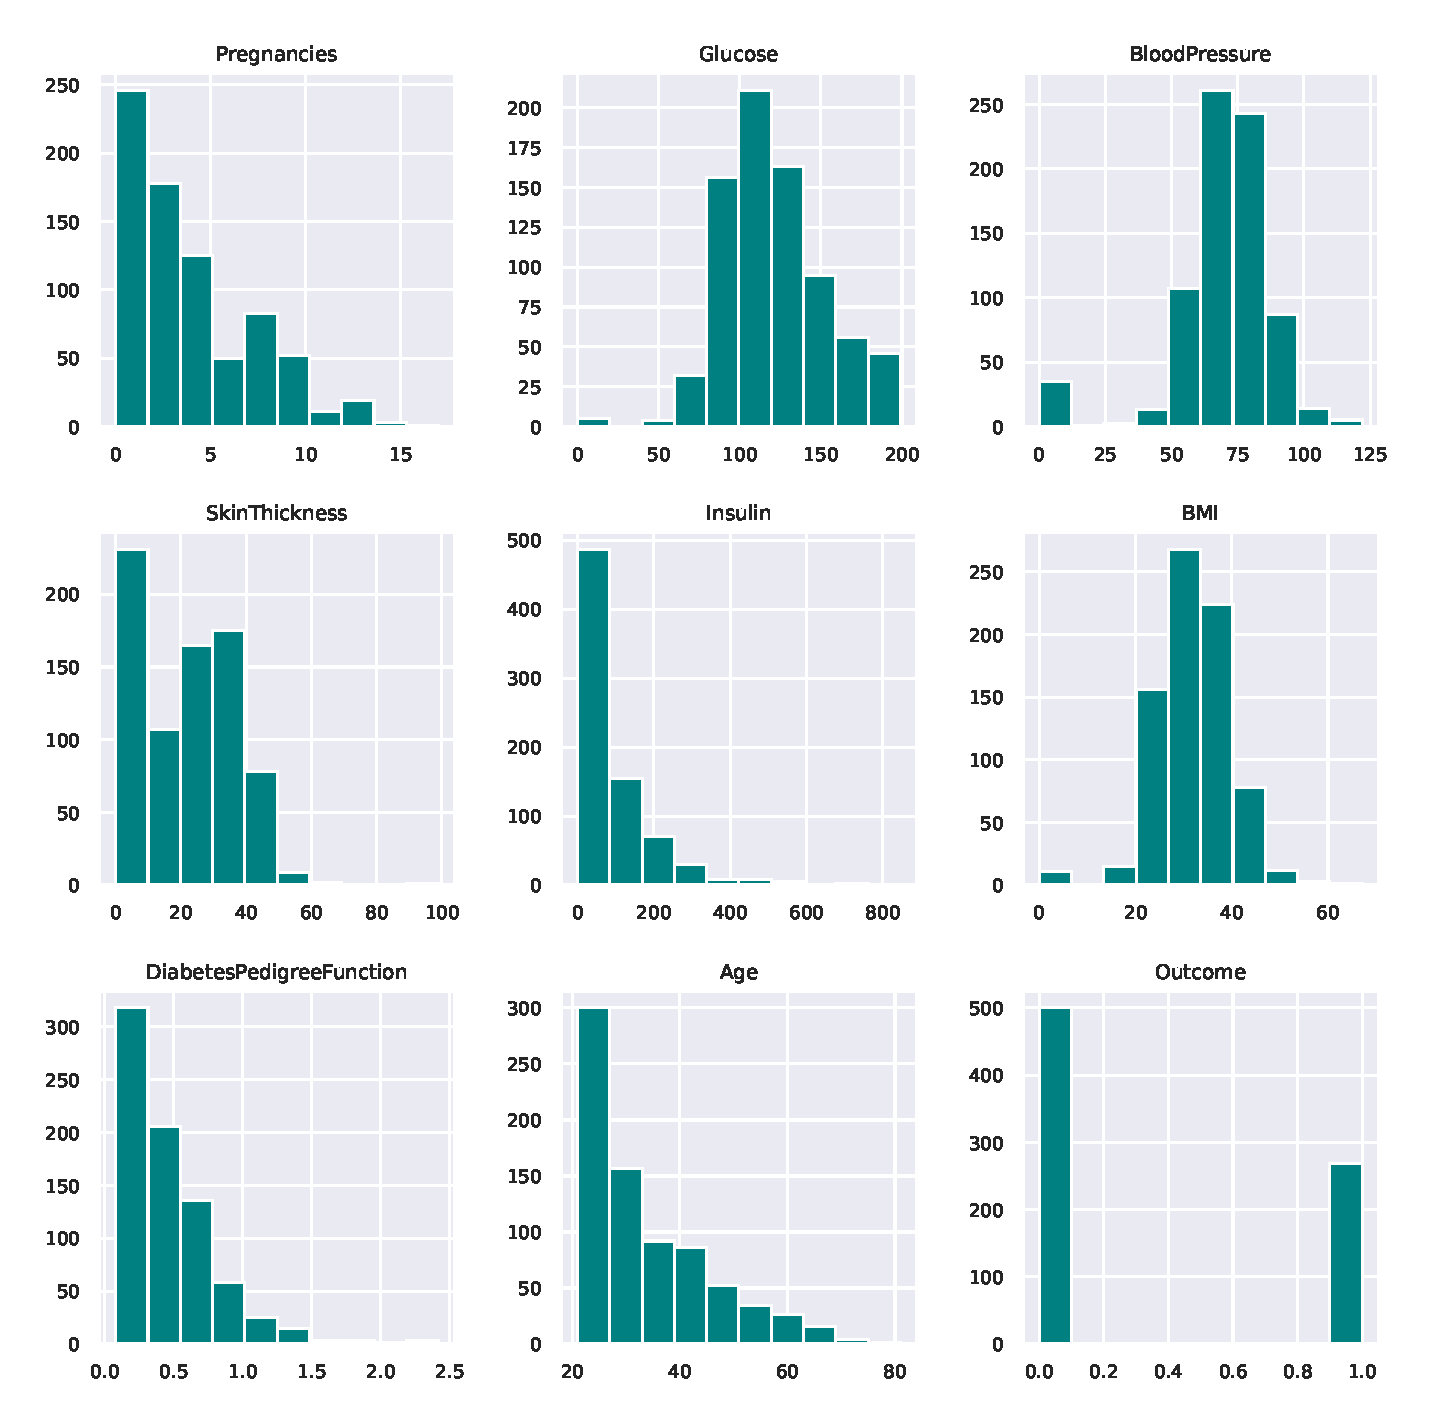
\includegraphics[height=\textwidth]{img/dataset_histogram.pdf}
			\caption{Histogram of the Dataset}
			\label{fig:datasetHistogram}
		\end{minipage}
	\end{figure}
	
	



	\subsection{Data preparation}
	The reading of the dataset is realised with multiples steps as shown in figure [\ref{methodsread}]. The raw data needs to be prepared in order to be applicable for all classification algorithm used in this project. All missing values, denoted with the value "0" needs to be replaced and the imbalanced of the dataset needs to be checked. To realized these steps, an Exploratory Data Analysis (EDA), shown in figure  [\ref{methodseda}] needs to be followed.
	\begin{figure}[H]
		\centering
		\begin{subfigure}[b]{0.49\textwidth}
			\centering
			
			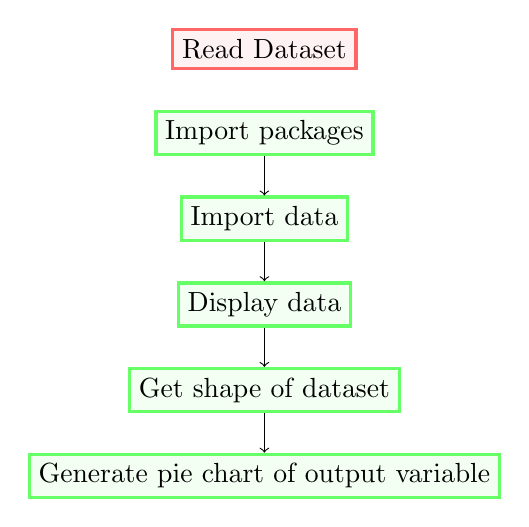
\begin{tikzpicture}[
				roundnode/.style={circle, draw=green!60, fill=green!5, very thick, minimum size=7mm},
				squarednode/.style={rectangle, draw=red!60, fill=red!5, very thick, minimum size=5mm},
				squarednode2/.style={rectangle, draw=green!60, fill=green!5, very thick, minimum size=5mm},
				node distance = 0.5cm,
				]
				%Nodes
				\node[squarednode](read){Read Dataset};
				\node[squarednode2](step0)[below=of read]{Import packages};
				\node[squarednode2](step1)[below=of step0]{Import data};
				\node[squarednode2](step2)[below=of step1]{Display data};
				\node[squarednode2](step3)[below=of step2]{Get shape of dataset};
				\node[squarednode2](step4)[below=of step3]{Generate pie chart of output variable};
				
				%Lines
				
				\draw[->] (step0.south) -- (step1.north);
				\draw[->] (step1.south) -- (step2.north);
				\draw[->] (step2.south) -- (step3.north);
				\draw[->] (step3.south) -- (step4.north);
				
			\end{tikzpicture}
			\caption{Reading dataset.}
			\label{methodsread}
		\end{subfigure}
		\begin{subfigure}[b]{0.49\textwidth}
			\centering
			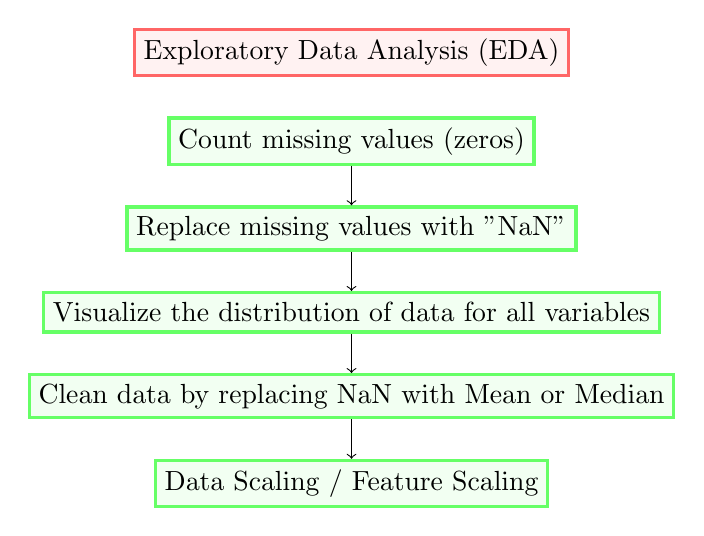
\begin{tikzpicture}[
				roundnode/.style={circle, draw=green!60, fill=green!5, very thick, minimum size=7mm},
				squarednode/.style={rectangle, draw=red!60, fill=red!5, very thick, minimum size=5mm},
				squarednode2/.style={rectangle, draw=green!60, fill=green!5, very thick, minimum size=5mm},
				node distance = 0.5cm,
				]
				%Nodes
				\node[squarednode](read){Exploratory Data Analysis (EDA)};
				\node[squarednode2](step0)[below=of read]{Count missing values (zeros)};
				\node[squarednode2](step1)[below=of step0]{Replace missing values with "NaN"};
				\node[squarednode2](step2)[below=of step1]{Visualize the distribution of data for all variables};
				\node[squarednode2](step3)[below=of step2]{Clean data by replacing NaN with Mean or Median};
				\node[squarednode2](step4)[below=of step3]{Data Scaling / Feature Scaling};
				
				%Lines
				
				\draw[->] (step0.south) -- (step1.north);
				\draw[->] (step1.south) -- (step2.north);
				\draw[->] (step2.south) -- (step3.north);
				\draw[->] (step3.south) -- (step4.north);
				
			\end{tikzpicture}   
			\caption{Exploratory Data Analysis (EDA)}   
			\label{methodseda}
		\end{subfigure}        
		\caption{Dataset import and preparation}

	\end{figure}

	

	First we have a look at the dataset to have an overview, shown in figure \ref{fig:datasetHistogram}. The summary of all variables is generated and gives useful information such as the number of entries, the mean, the standard deviation, the minimum value, the quartiles, and the maximum value. shown in figure \ref{fig:distributionBoxplot}.
	\medbreak
	The output variable is shown in figure \ref{fig:outcome}. This variable is assumed to be exact in the sense that their is no false positive nor false negative. From this statement, the goal is to reach the exact same output using all the predictors given in the dataset.
	\medbreak
	By looking at the data in table \ref{tab:nullValues}, it is easy to see that some "0" values do not make sense. For example, a value of zero in the BMI or in the Blood pressure variable would indicate that the patient is not existing or dead. The replacement of the zero values is made by first analyzing the distribution of the data. If the distribution is symmetric, the missing values are replaced with the mean value. If the distribution shows a lot of outliners, the missing values are replaced by the median value. The distribution and box plots are generated (see figure \ref{fig:distributionBoxplot}) to permit the decision. Once the missing values are replaces, those figures are re-generated to assure a similar distribution as before the cleaning. Table \ref{tab:nullValues} shows the amount of the "0" values and how they were handled.

	\begin{table}[H]
		%\renewcommand{\arraystretch}{1.3}
		\centering
		\begin{tabular}{lcc}
			Data column & Amount of "0" values & Chosen replacement method \\
			\toprule
			Pregnancies          &         0 &  None \\
 			Glucose              &         5 & Mean \\
			Blood Pressure        &        35 & Mean \\
			Skin Thickness        &       227 & Median\\
			Insulin              &       374  & Median\\
			BMI (Body Mass Index) &        11 & Median \\
			Diabetes Pedigree Function  &    0 & None \\
			Age                  &         0 & None \\
		\end{tabular}
		\caption{Amount of zero values in dataset}
		\label{tab:nullValues}
	\end{table}
%	\subsubsection{Dataset Splitting}
%	The dataset needs to be split into a test dataset and a training dataset to train and test the machine learning models. In our case, the test dataset is 25\% of the entire dataset. We use the training dataset to fit the machine learning model and the test dataset to evaluate the machine learning model.  When we split a dataset, there are two competing concerns. Our parameter estimates have more significant variance if we have less training data, and our performance statistics will have more significant variance if we have less testing data. Therefore the 25\% is an excellent choice and the default in scikit-learn library. 
%	\medbreak
%	Both sets will be further split into an x-set and a y-set, where the y-set contains the outcome, if a person has diabetes or not (True or False), the x set contains all measured patient data. If the model is fitted with the training set, the test set will evaluate the model performance.
	% Data Scaling / Feature Scaling
	\subsubsection{Data Scaling / Feature Scaling}
	Data scaling or feature scaling is used in some machine learning algorithms. If there is a vast difference between numbers sizes, the model could assume that bigger numbers are more significant than smaller ones. Therefore all values are normalized or standardized.
	\medbreak
	In our case, data scaling was used for the LR, SGD, SVMs and KNN algorithms, in all cases, the scaled data had better accuracy than the non-scaled data. Data scaling also helps some models (for example, SGD) with the training time, significantly improving the converge time.
	
	% Imbalanced Data
 	\subsubsection{Imbalanced Data}
 	The Pima Indians Diabetes Database \cite{Pima} is quite imbalanced. This can be seen in figure \ref{fig:outcome}, the outcome has way more non-diabetes patients (diabetes:  34.9\%, No diabetes: 65.1\%) than patients with diabetes. Some algorithms have problems with imbalanced data, for example, the SVMs algorithm. Suppose the imbalanced data are not handled in the SVMs algorithm. It will predict every patient as a non-diabetes patient and, therefore, have a pretty good accuracy because 65.1\% of the patients are non-diabetic. This gives us a specificity of 100\% and a sensitivity of 0\%. Therefore, the model is useless. The imbalanced data need to be checked and handled if the algorithm requires it.
	
	\begin{figure}[H]
		\begin{minipage}[b]{0.65\textwidth}
			\centering
			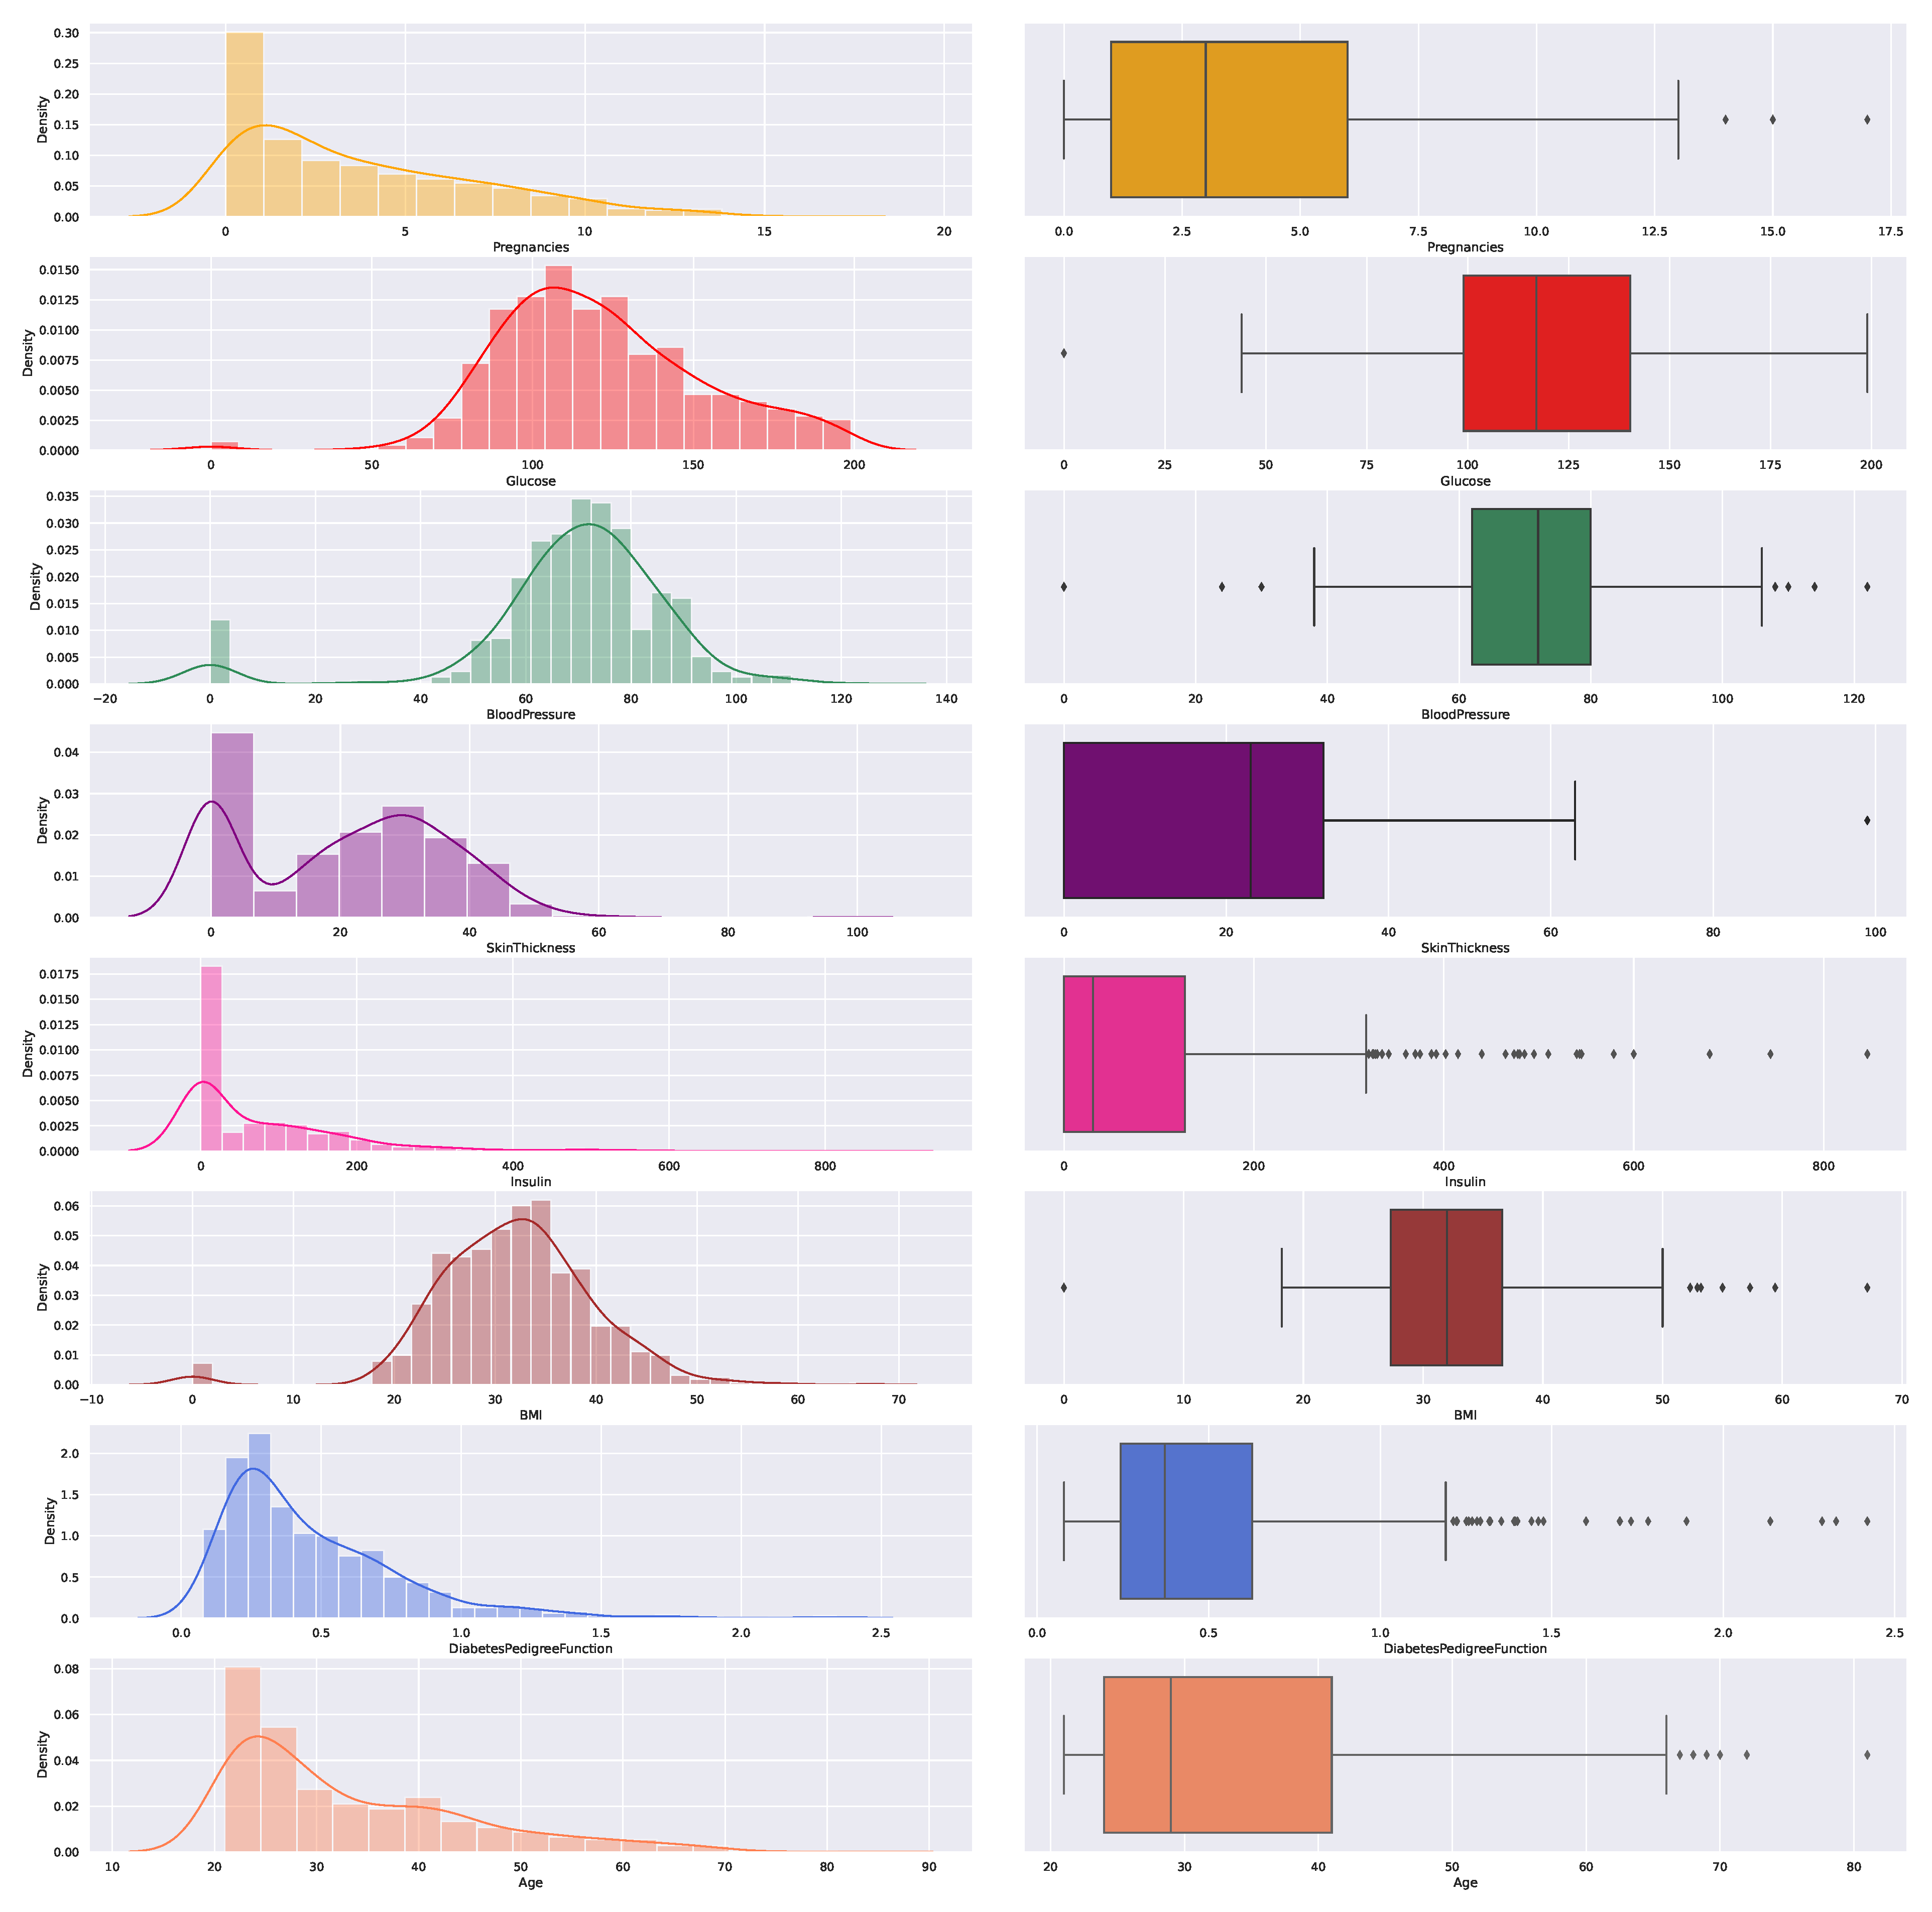
\includegraphics[width=\textwidth]{img/dataset_distibutionAndBoxPlot.pdf}
			\caption{Dataset distribution and boxplots}
			\label{fig:distributionBoxplot}
		\end{minipage}
		\begin{minipage}[b]{0.35\textwidth}
			\centering
			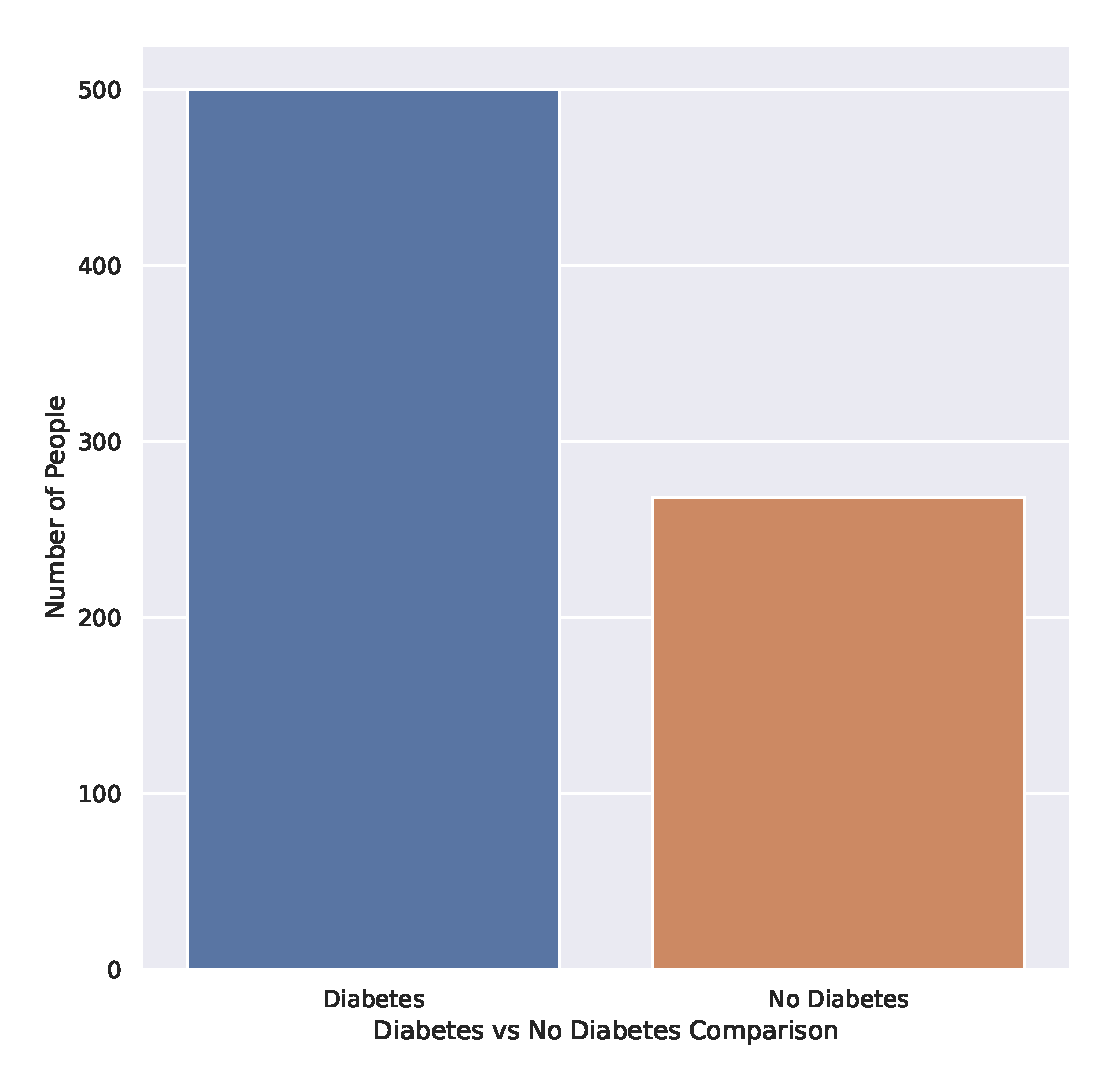
\includegraphics[width=\textwidth]{img/dataset_diabetes_and_non_diabetes.pdf}
			\caption{Dataset Outcome}
			\label{fig:outcome}
		\end{minipage}
	\end{figure}

	%% RESULTS
	\section{Results}
	We applied the mentioned machine learning algorithms and got the performance results in the table \ref{fig:results}, and for the accuracy and f1 score, boxplots were made, see figure \ref{fig:modelComparision}.

	\begin{table}[H]
		\renewcommand{\arraystretch}{1.3}
		\begin{tabularx}{\linewidth}{lXXXX}
			Model & Accuracy & Specificity & Sensitivity & F1 \\
			\toprule
			Decision Trees  &  0.708502  &  0.715447  &  0.608696  &  0.570121  \\
			K Nearest Neighbors  &  0.740216  &  0.861789  &  0.565217  &  0.619996  \\
			Logistic Regression  &  0.765992  &  0.853659  &  0.565217  &  0.614503  \\
			Naive Bayes  &  0.729555  &  0.772358  &  0.666667  &  0.619294  \\
			Support Vector Machines  &  0.718489  &  0.617886  &  0.724638  &  0.625714  \\
			Stochastic Gradient Descent  &  0.745344  &  0.569106  &  0.869565  &  0.493682  \\
		\end{tabularx}
		\caption{Model Performance Results}
		\label{fig:results}
	\end{table}
	\begin{figure}[H]
		\centering
		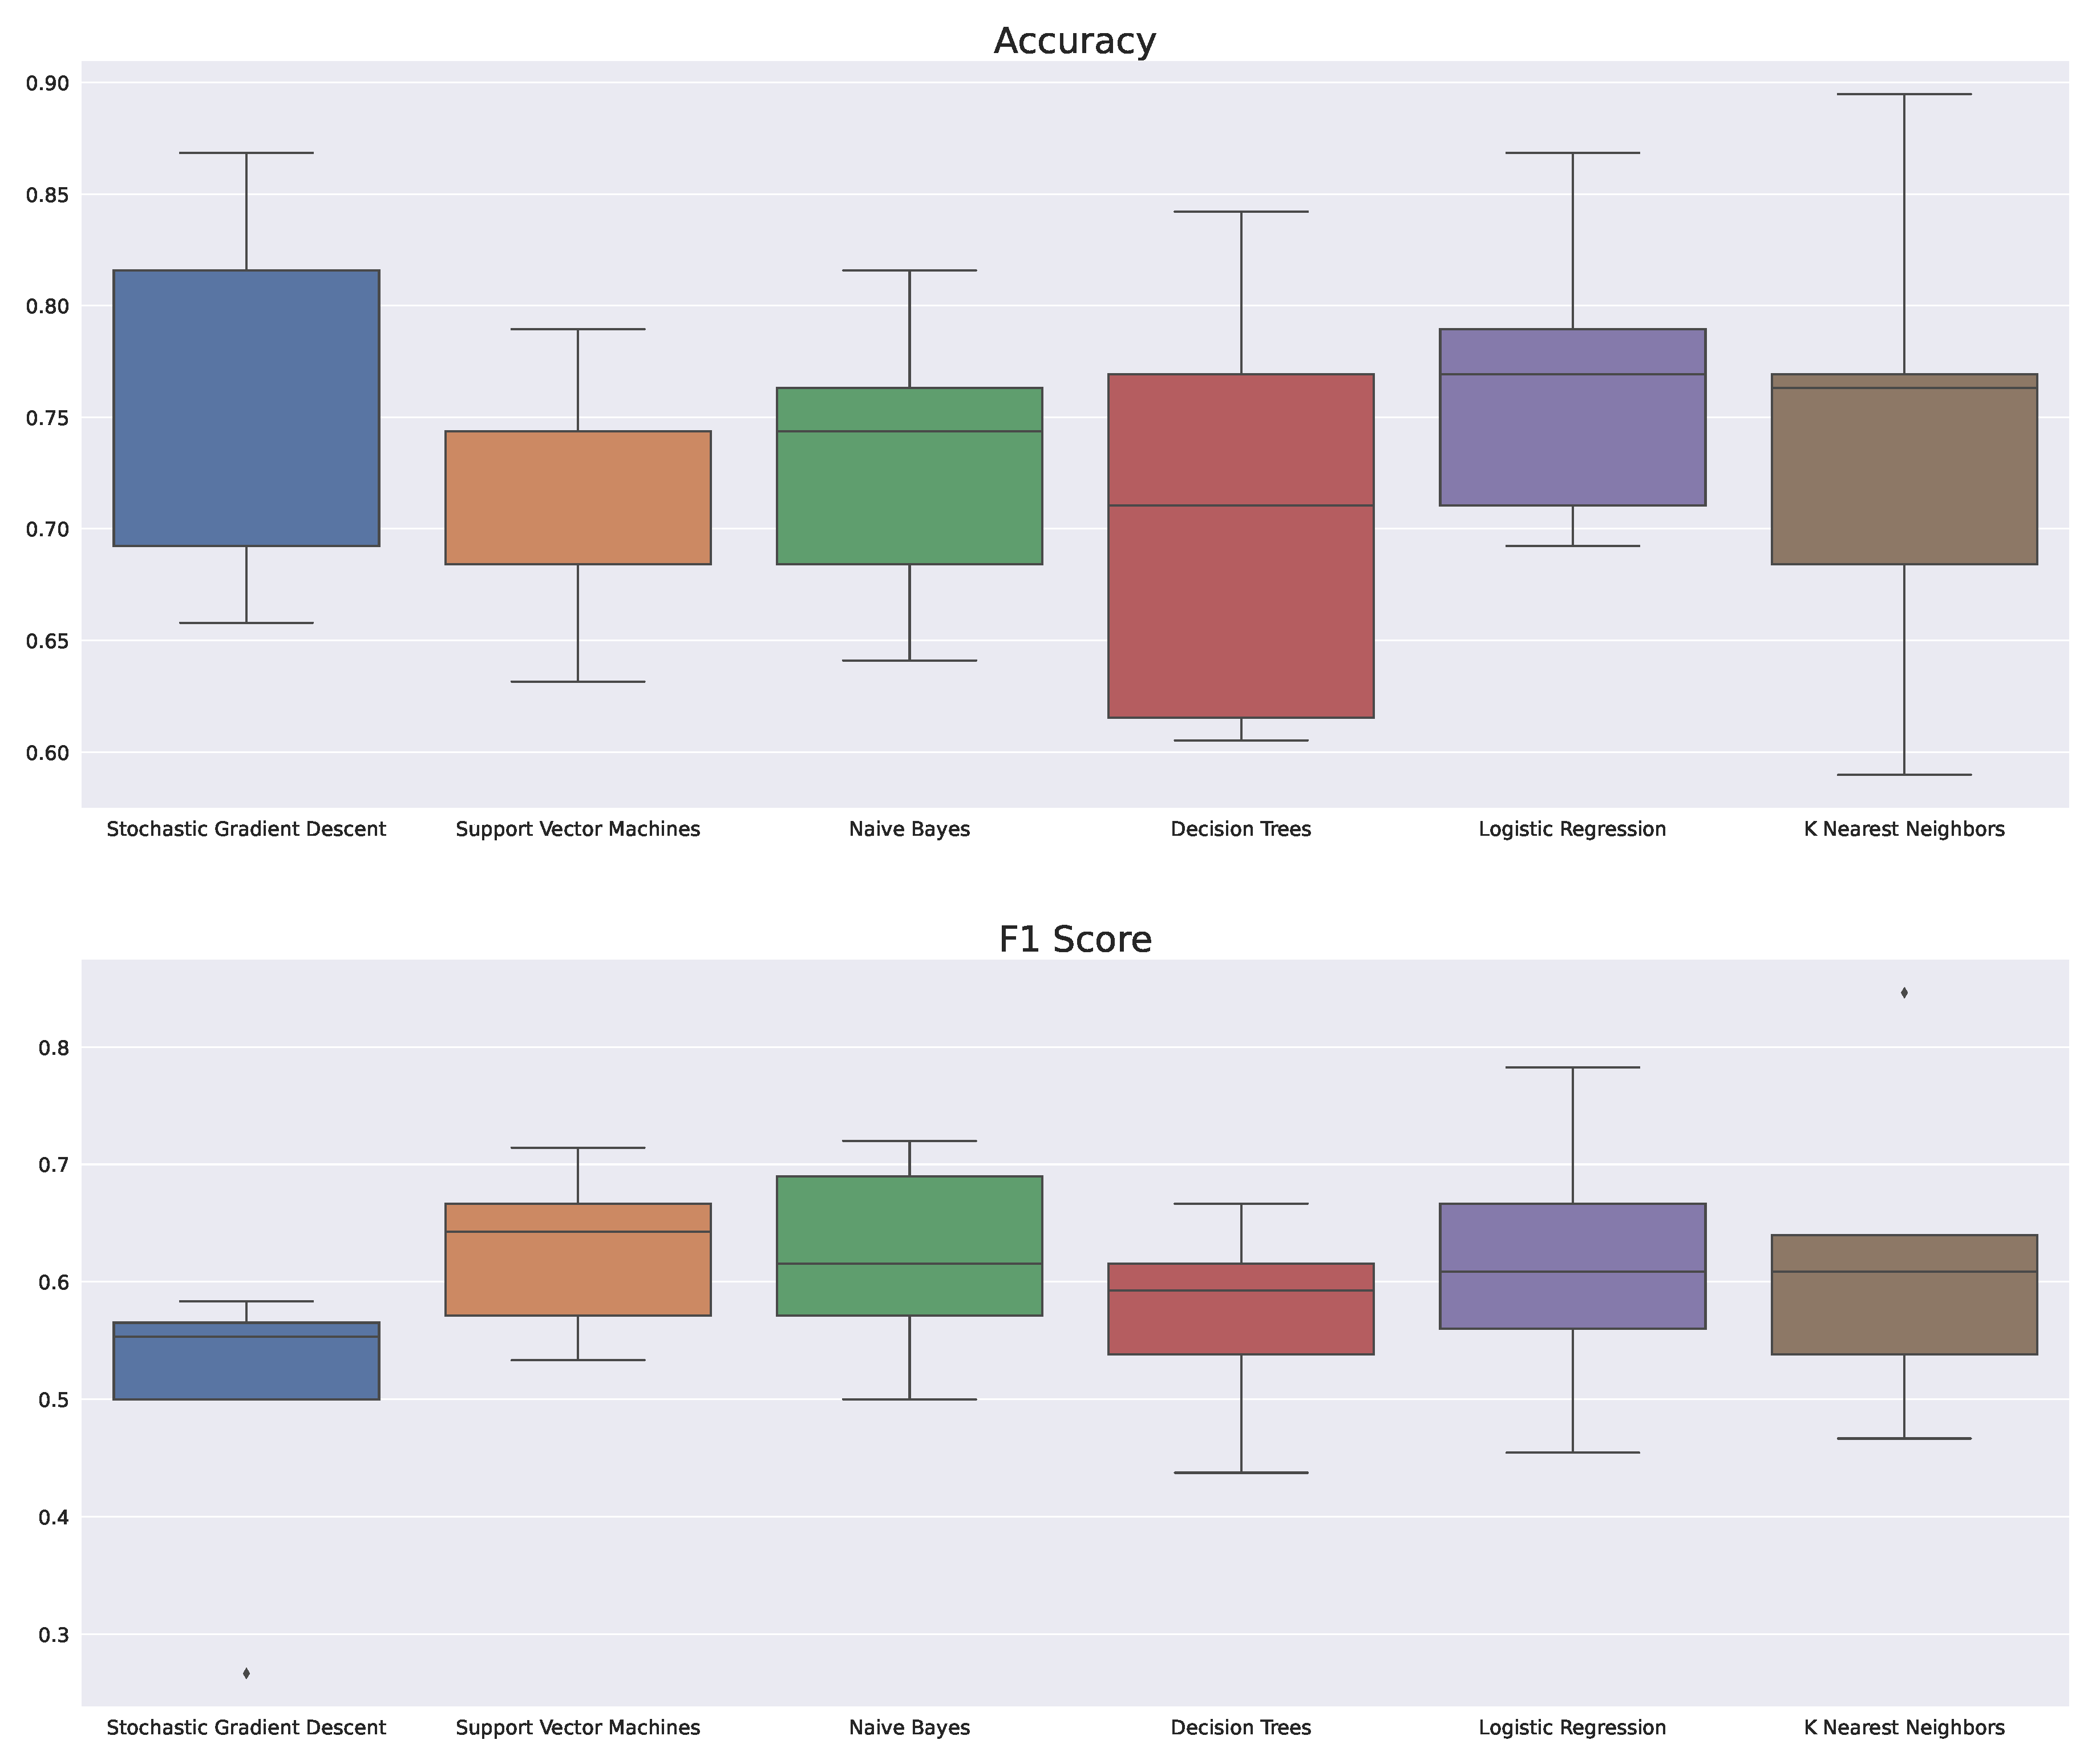
\includegraphics[width=0.8\textwidth]{img/model_comparision.pdf}
		\caption{Model Comparison}	
		\label{fig:modelComparision}
	\end{figure}
	The overall best model is the one with the Logistic Regression algorithm.


	%% DISCUSSION
	\section{Discussion}
	Diabetes is a well-knows chronic metabolic disease that results from defects in insulin secretion, insulin action, or both. The long-term complications related to diabetes could be critical. To avoid dramatic situations, the diagnosis of diabetes should be made as early as possible. To this day, Prediction Analysis as been used to assist medical decision-making. What differs between each algorithm used to predict disease such as diabetes is the accuracy find in the evaluation metrics. By evaluating the accuracy of multiple algorithms, one can find the one that suits the most in a medical application such as diabetes diagnosis. In order to do this comparison, the Pima Indian Diabetes Database is prepared and applied to classification algorithms such as Logistic Regression, Naïve Bayes, Stochastic Gradient Descent, K-Nearest Neighbors, Decision Tree, and Support Vector Machine. The result shows that the best accuracy is reached with \hl{[???????]} with an accuracy of \hl{[???????]}. The result is explained by a good ratio of number of correct predictions to the total number of input samples. The database includes only woman and is therefore limited to female diagnosis only. Future work could include a study of male-diagnosed patient to develop a more inclusive diagnosis method.

	\hl{TODO -> a ccuracy of arounf 77\% is really bad not? its a bit better than guessing, shall we write something about that? WHO criteria of $\geq$80\% sensitivity and $\geq$97\% specificity -> example requirments who coivd tests}
	

\printbibliography
\end{document}